\begin{figure}[htp] \centering
    \begin{subfigure}[b]{0.48\columnwidth}
        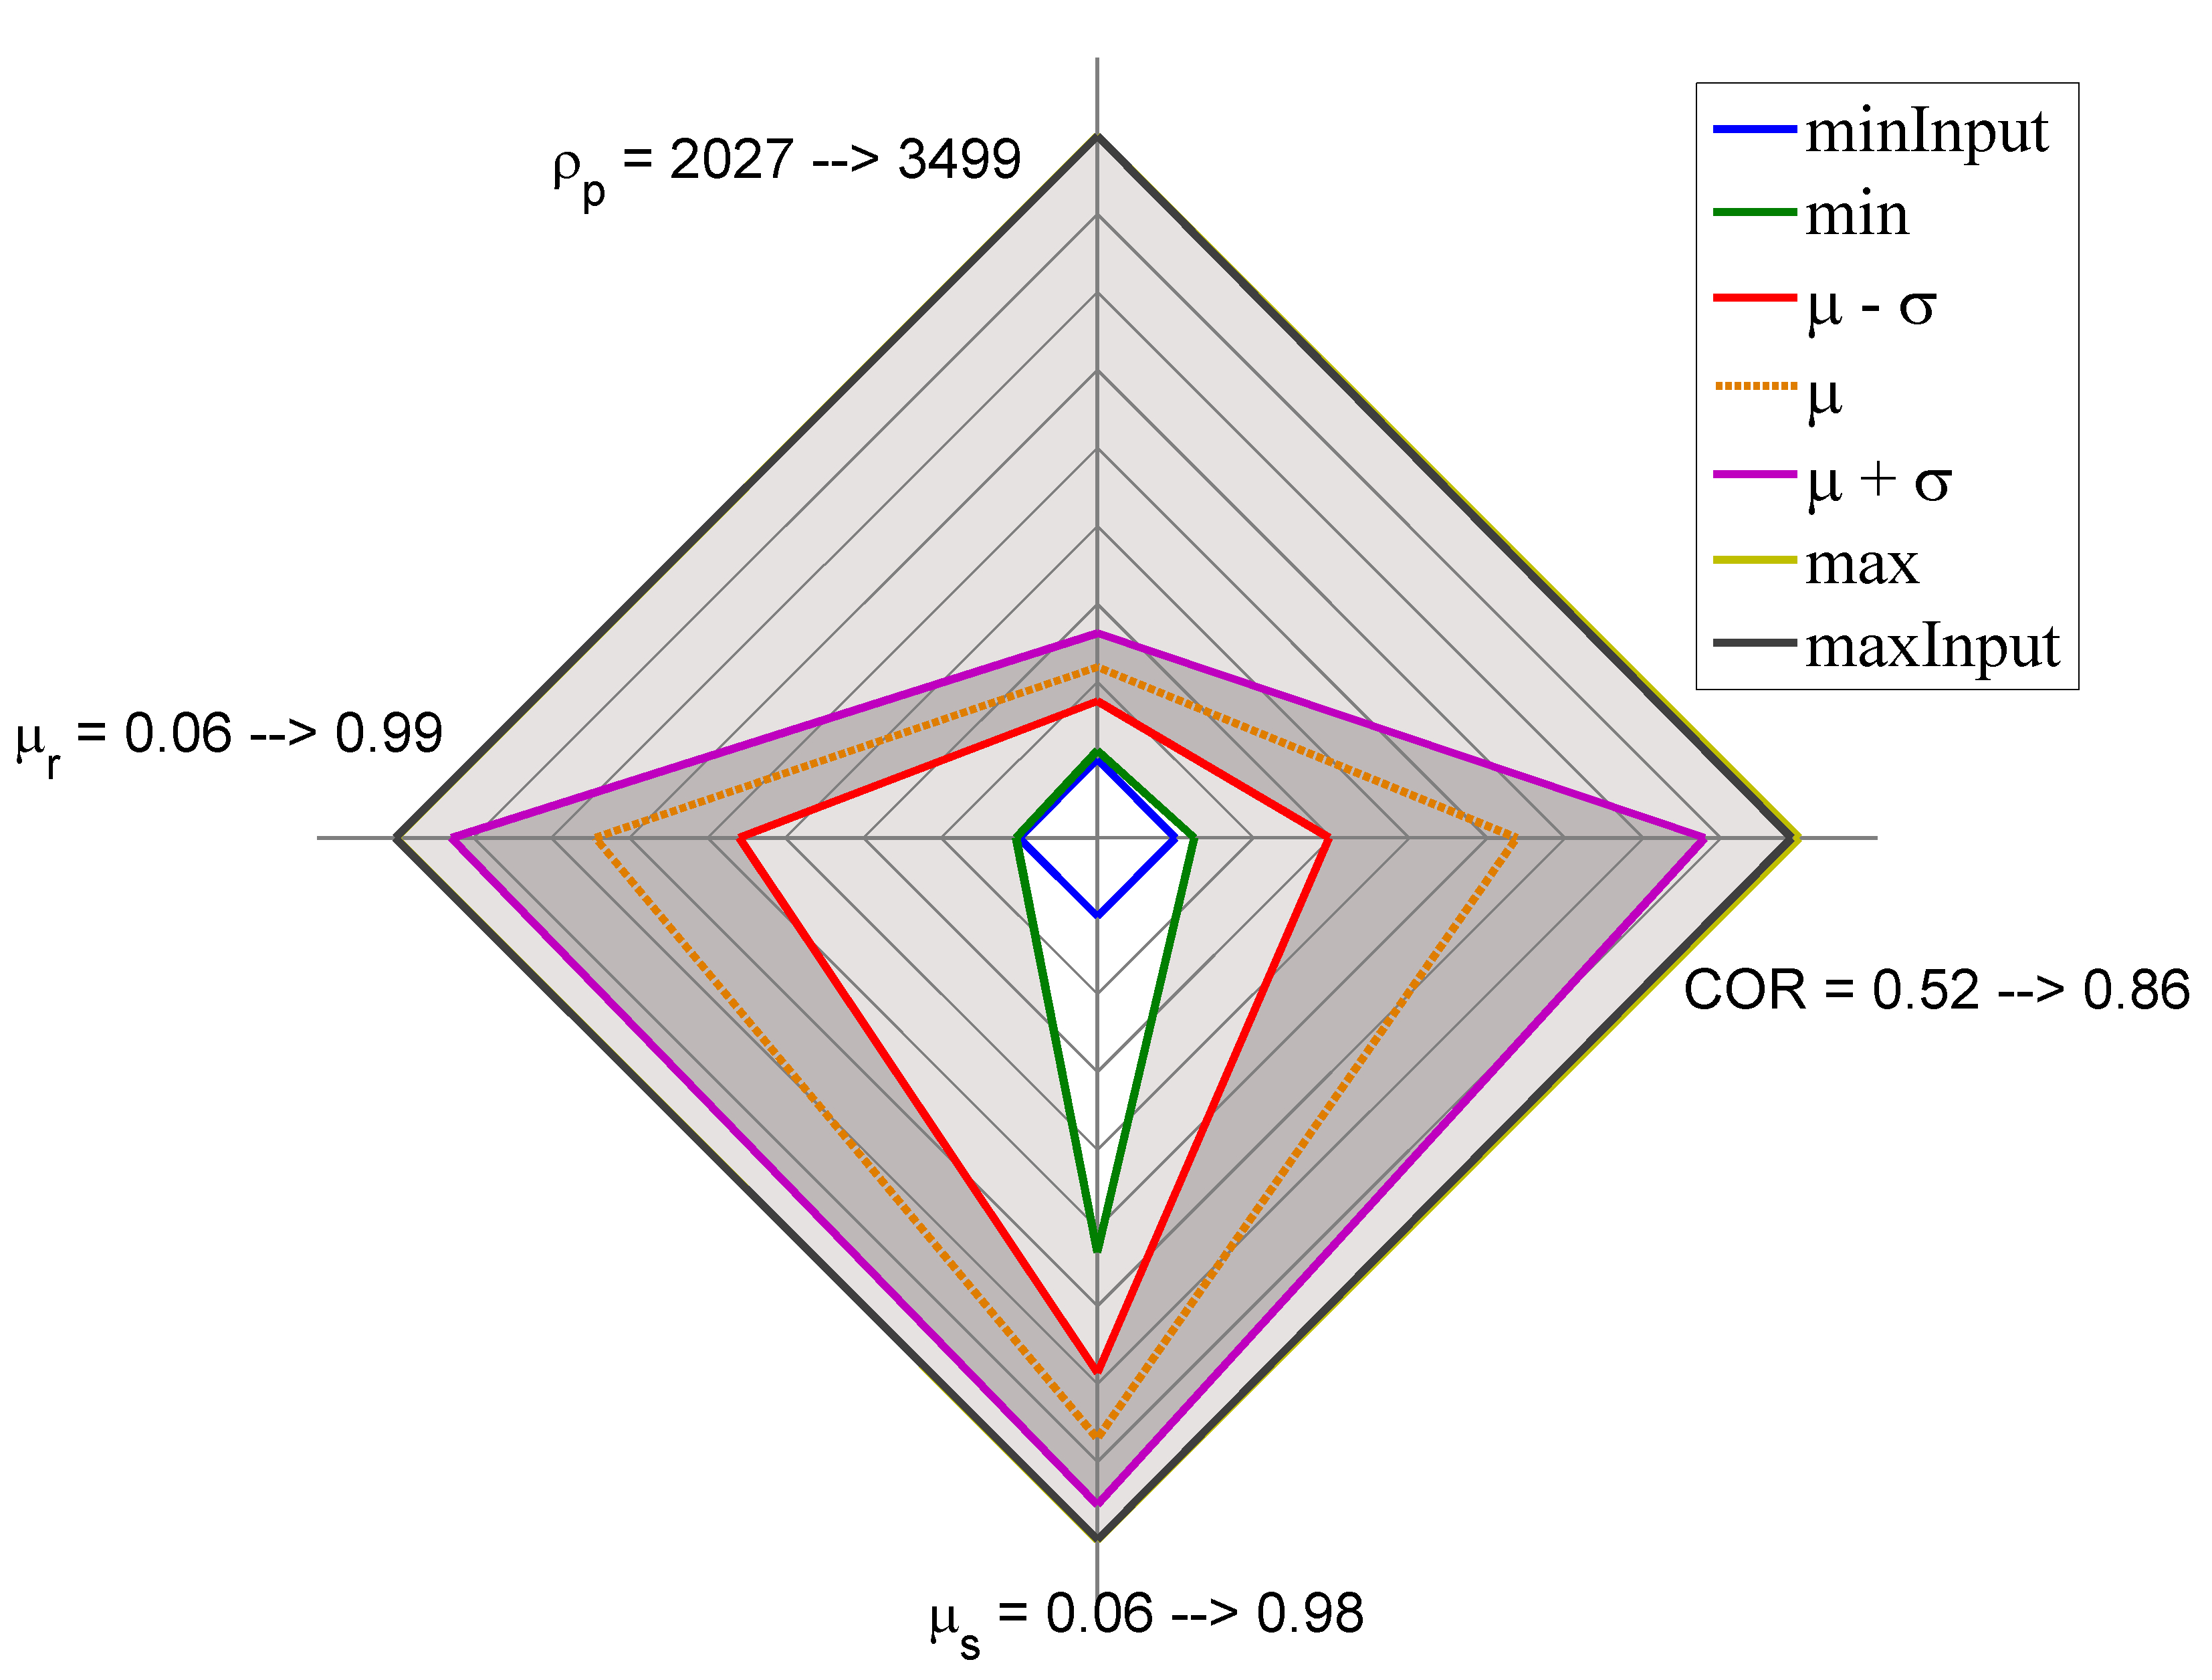
\includegraphics[width=\textwidth]{images/original/24radarpirker1schulze10070}
        \caption{Radar P1 Schulze10070}
        \label{fig:24radarpirker1schulze10070}
    \end{subfigure}
    \begin{subfigure}[b]{0.48\columnwidth}
        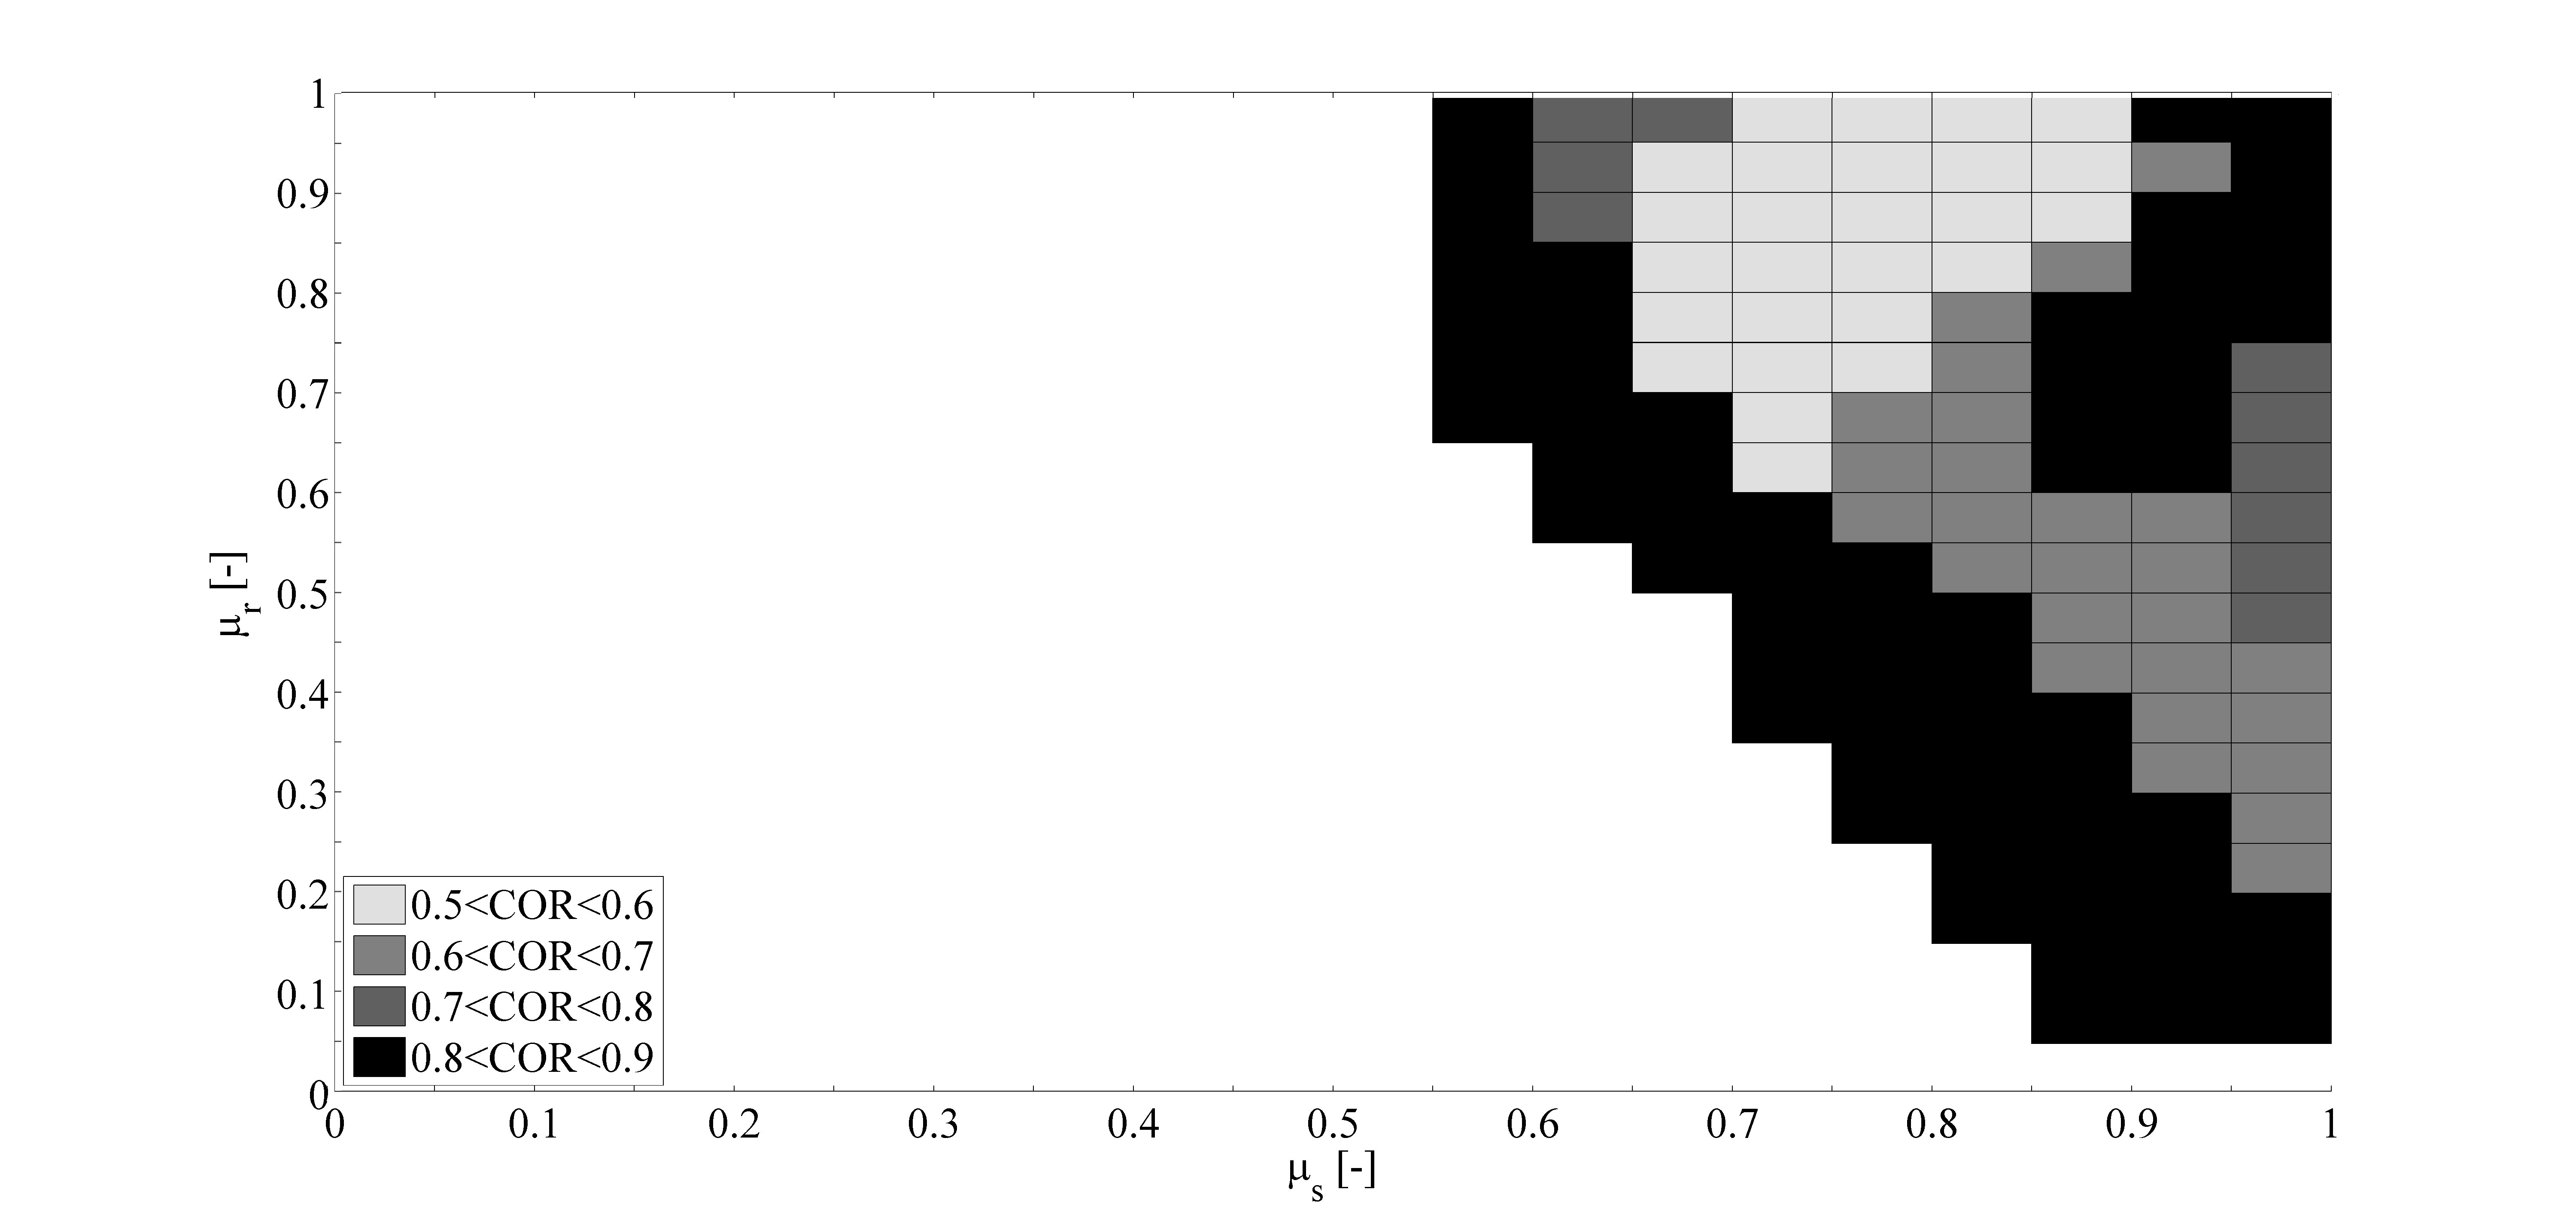
\includegraphics[width=\textwidth]{images/original/25cloudpirker1schulze10070}
        \caption{Cloud P1 Schulze10070}
        \label{fig:25cloudpirker1schulze10070}
    \end{subfigure}\\
        \begin{subfigure}[b]{0.48\columnwidth}
        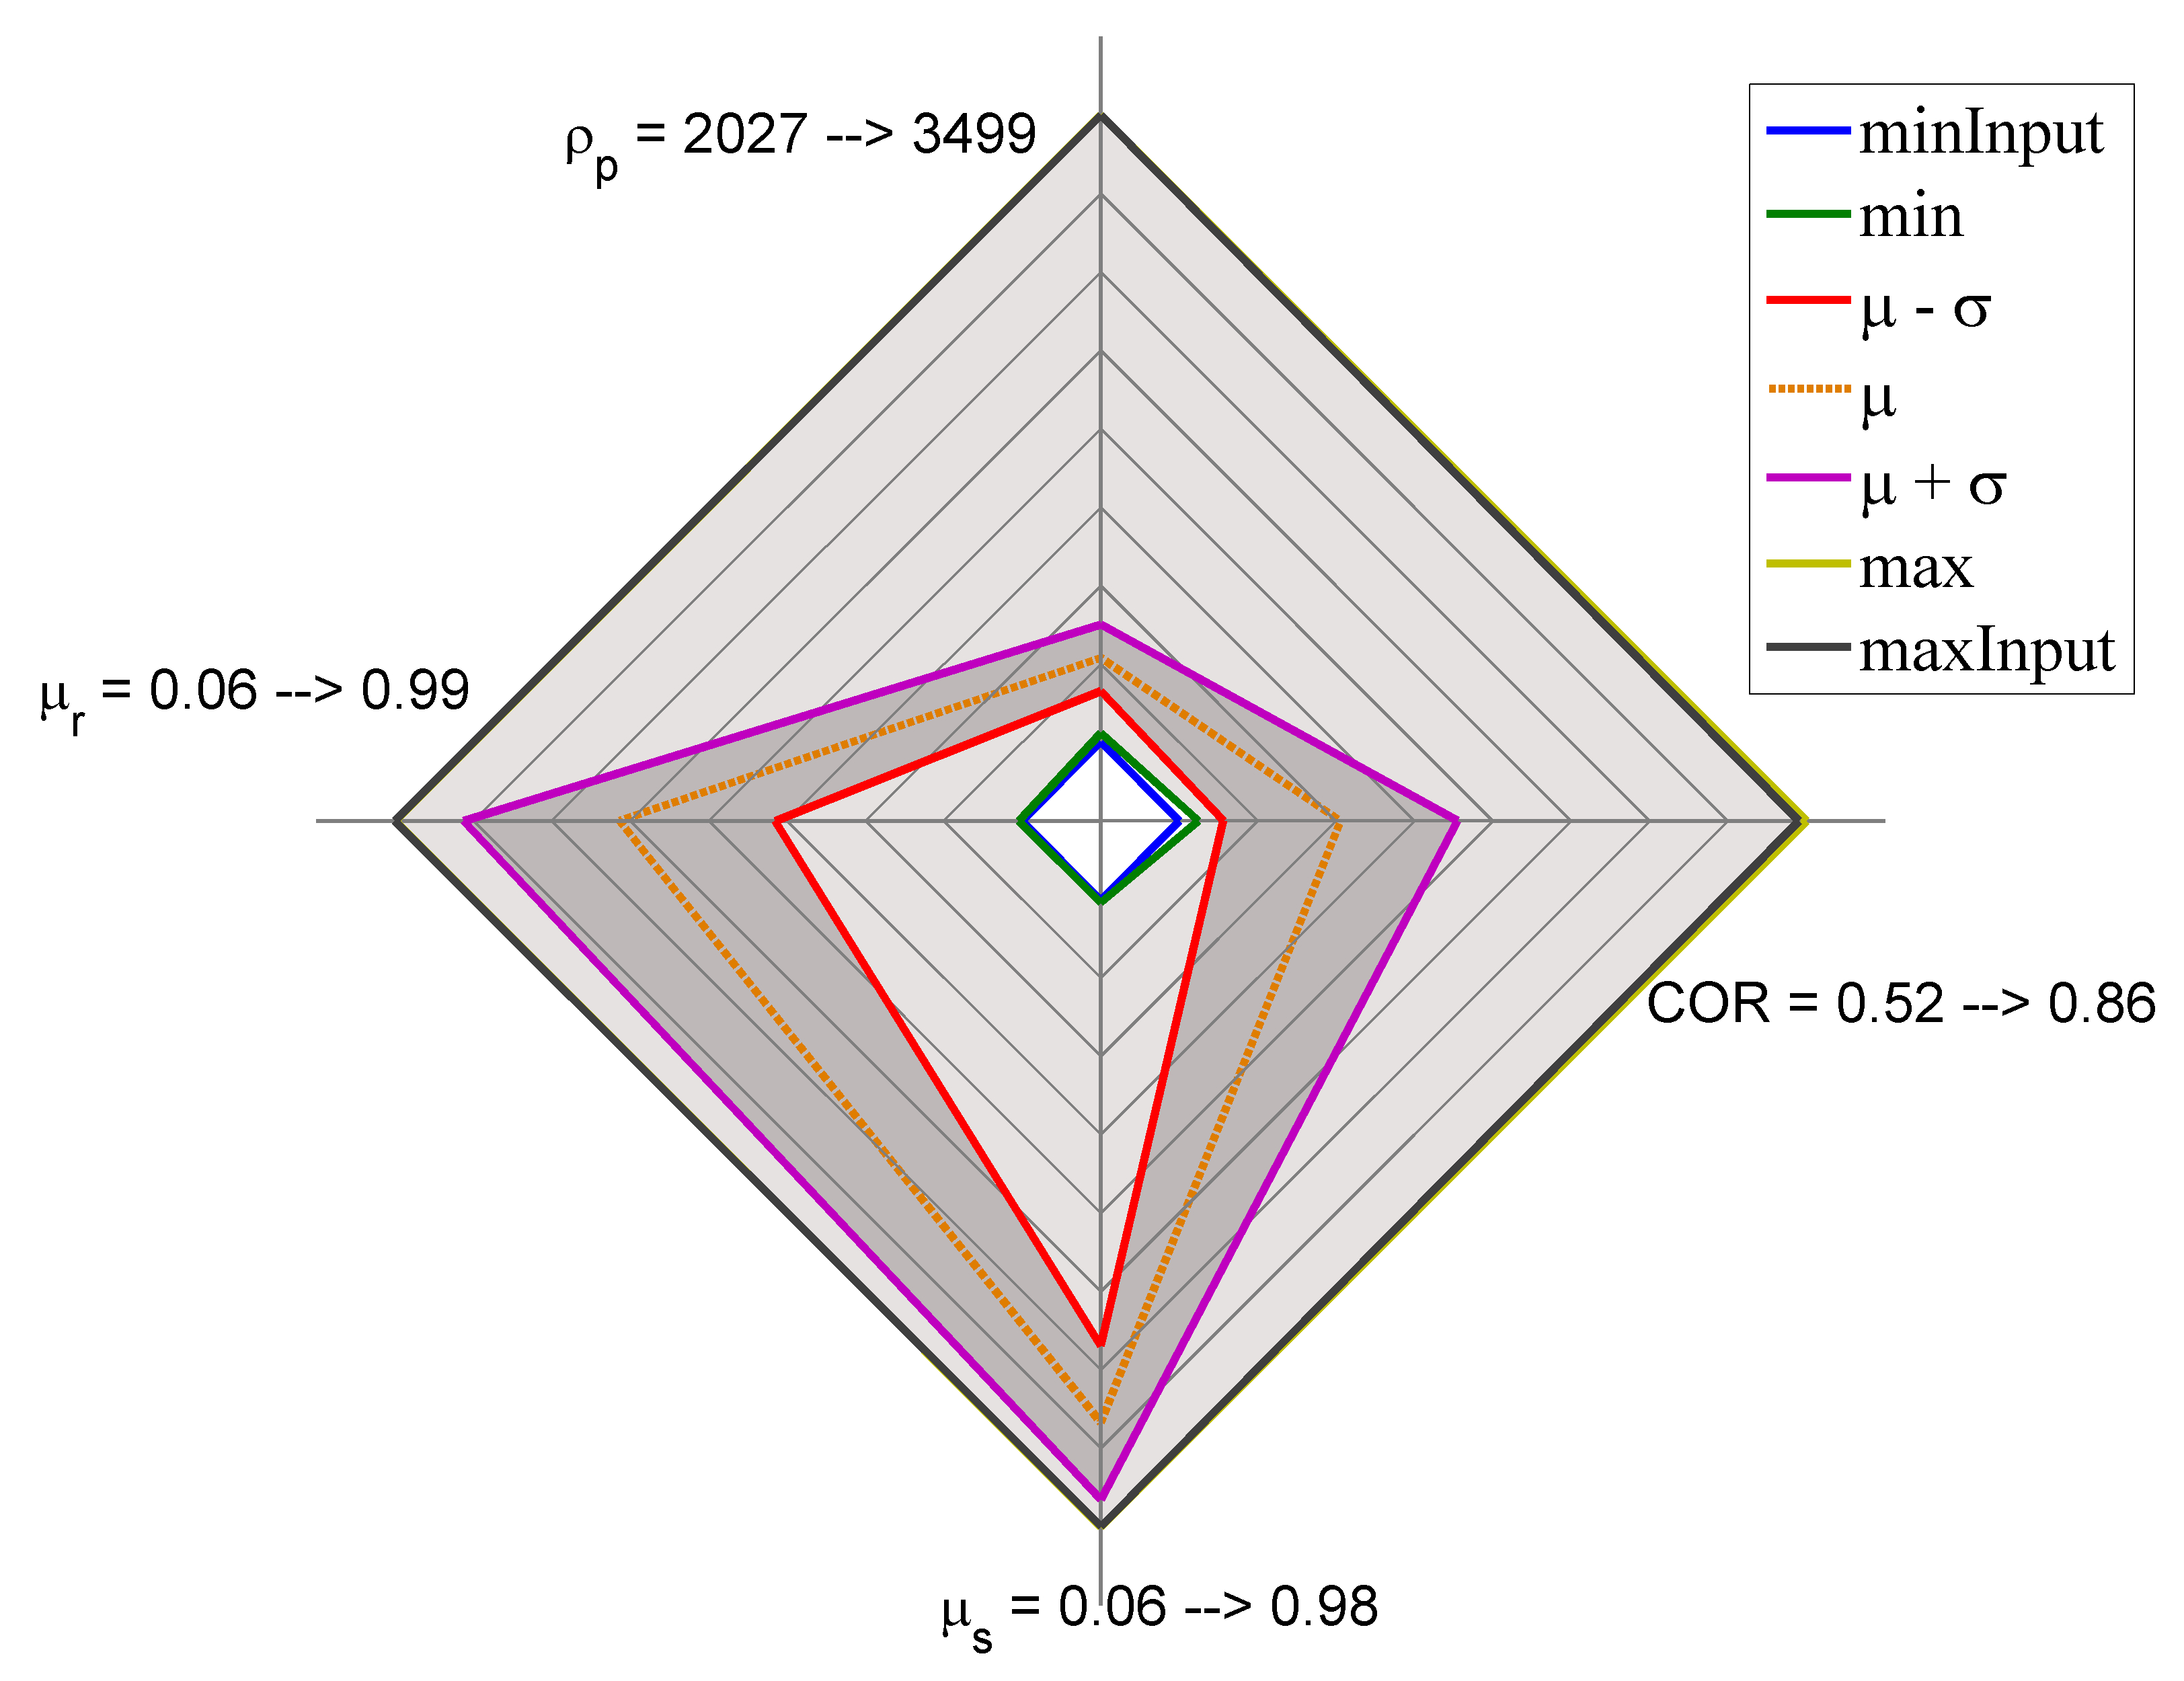
\includegraphics[width=\textwidth]{images/original/26radarpirker08schulze10070}
        \caption{Radar P08 Schulze10070}
        \label{fig:26radarpirker08schulze10070} 
    \end{subfigure}
    \begin{subfigure}[b]{0.48\columnwidth}
        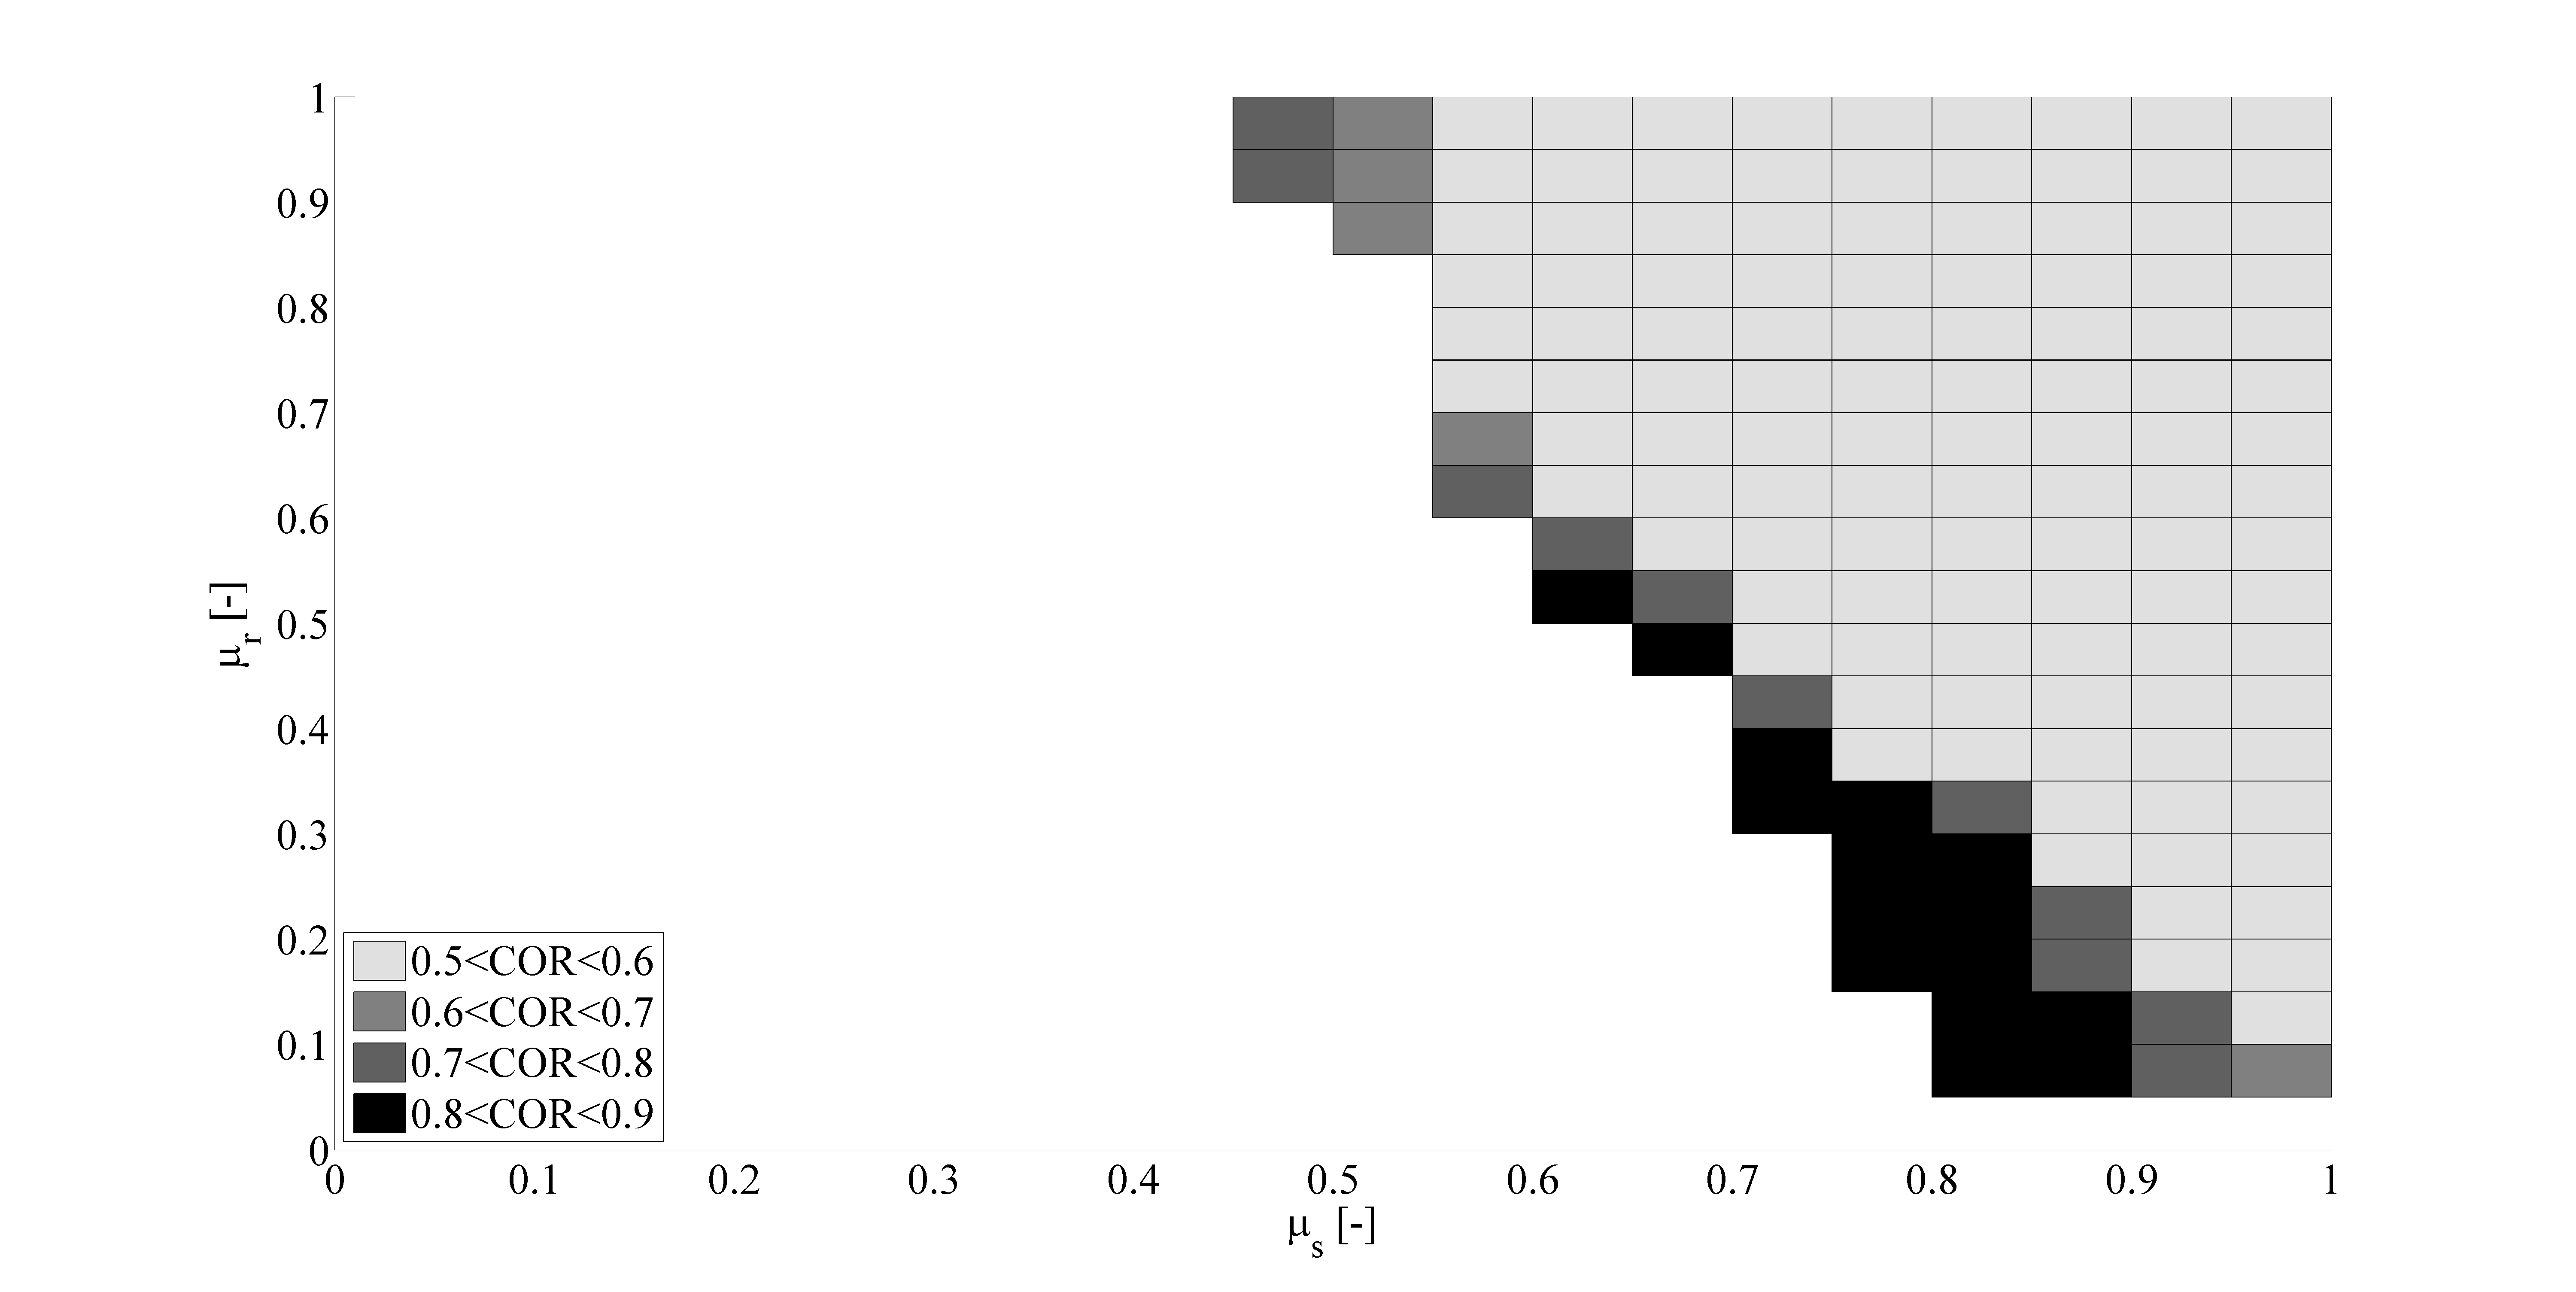
\includegraphics[width=\textwidth]{images/original/27cloudpirker08schulze10070}
        \caption{Cloud P08 Schulze10070}
        \label{fig:27cloudpirker08schulze10070} 
    \end{subfigure}\\
        \begin{subfigure}[b]{0.48\columnwidth}
        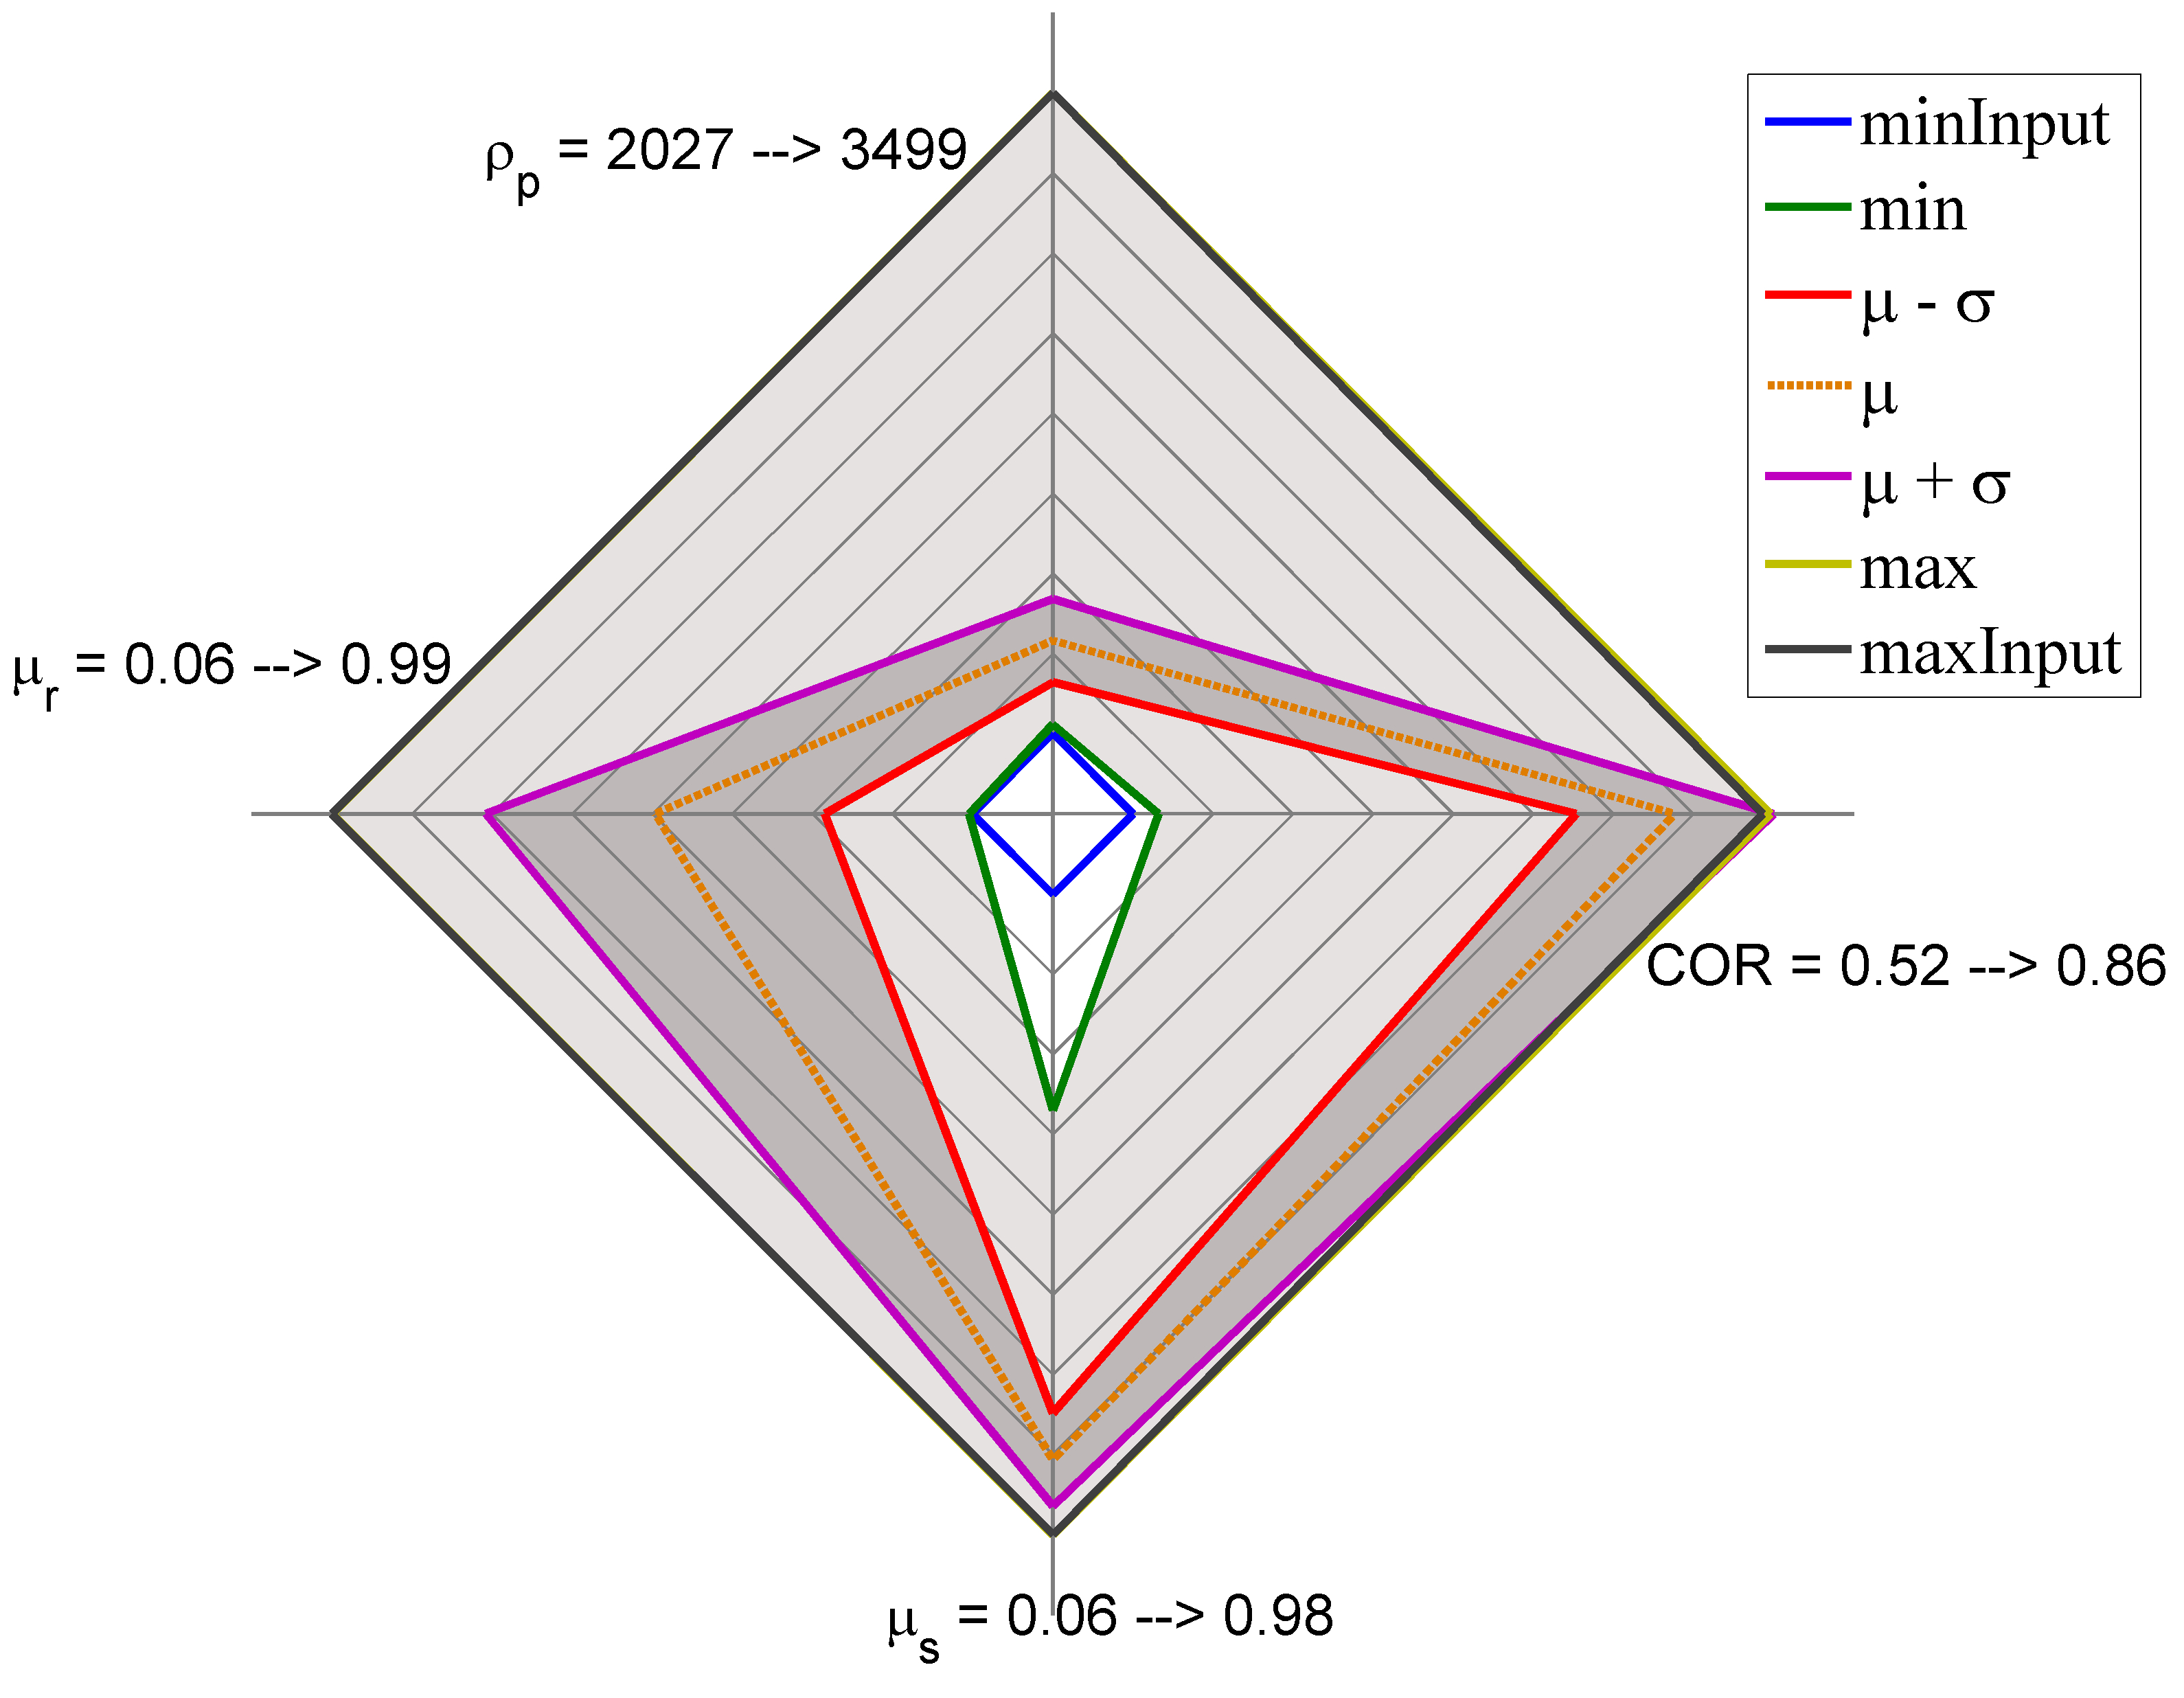
\includegraphics[width=\textwidth]{images/original/28radarpirker12schulze10070}
        \caption{Radar P12 Schulze10070}
        \label{fig:28radarpirker12schulze10070} 
    \end{subfigure}
    \begin{subfigure}[b]{0.48\columnwidth}
        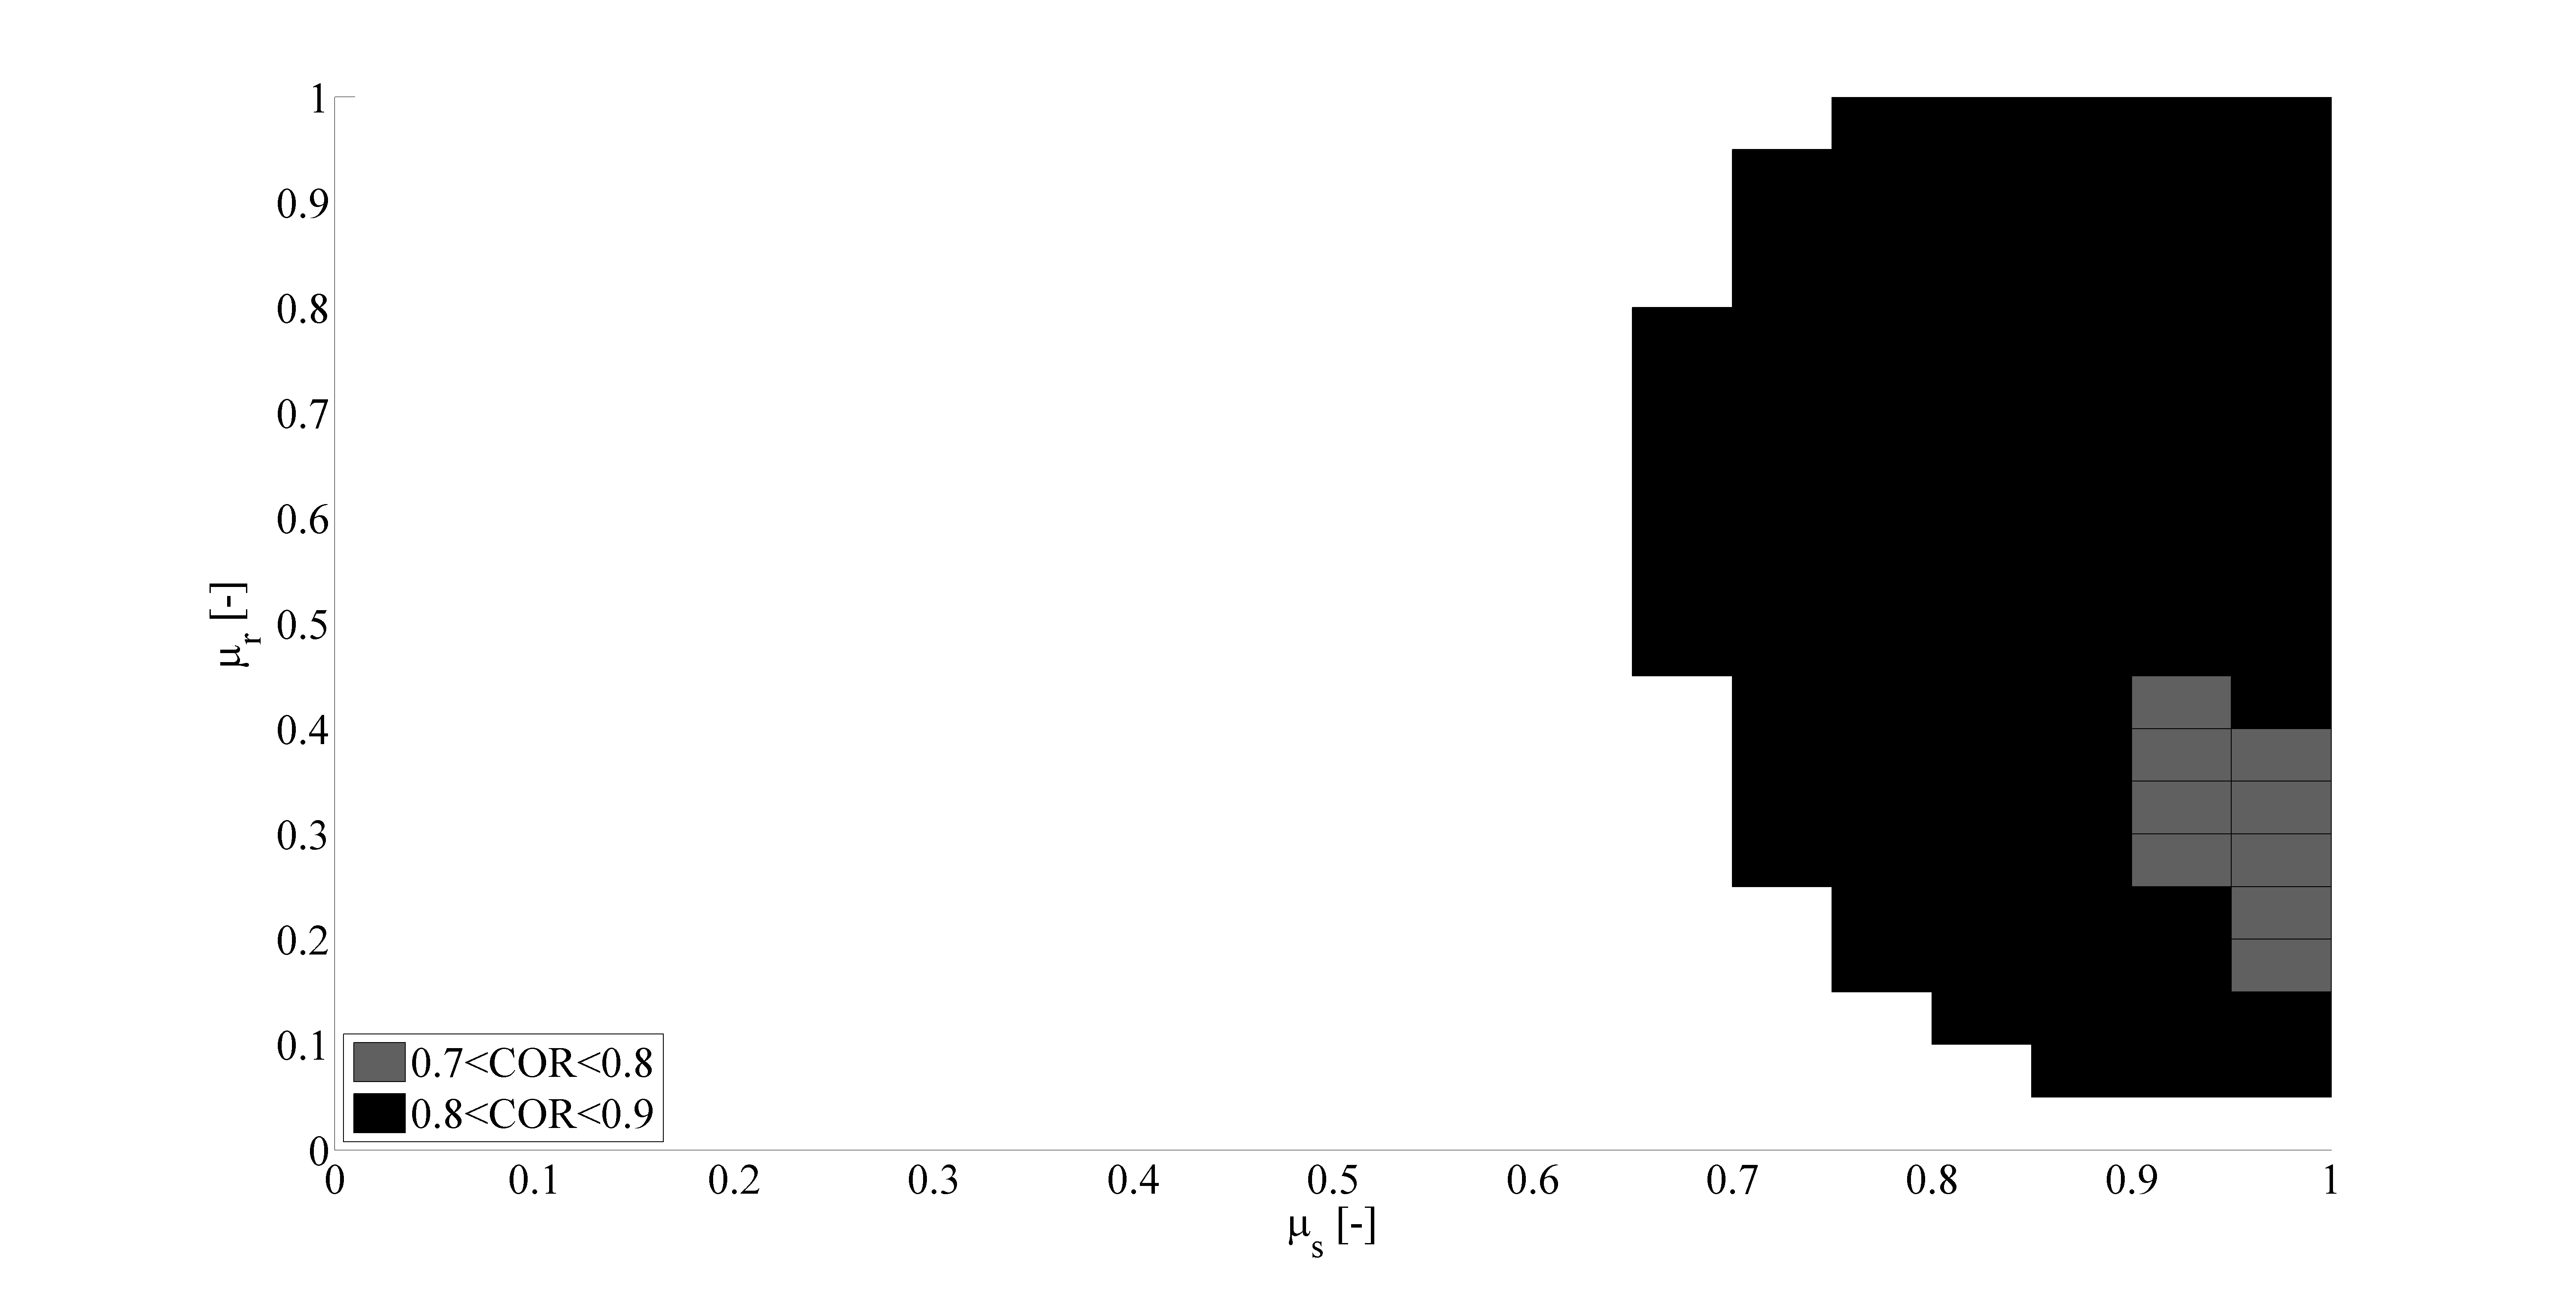
\includegraphics[width=\textwidth]{images/original/30cloudpirker12schulze10070}
        \caption{Cloud P12 Schulze10070}
        \label{fig:30cloudpirker12schulze10070} 
    \end{subfigure}
    \caption{Comparison between the original experimental selection P=1 and the
    increased and decreased results.}
    \label{fig:29schulzeradarandcloud}
\end{figure}